%package list
\documentclass{article}
\usepackage[top=3cm, bottom=3cm, outer=3cm, inner=3cm]{geometry}
\usepackage{multicol}
\usepackage{graphicx}
\usepackage{url}
%\usepackage{cite}
\usepackage{hyperref}
\usepackage{array}
%\usepackage{multicol}
\newcolumntype{x}[1]{>{\centering\arraybackslash\hspace{0pt}}p{#1}}
\usepackage{natbib}
\usepackage{pdfpages}
\usepackage{multirow}
\usepackage[normalem]{ulem}
\useunder{\uline}{\ul}{}
\usepackage{svg}
\usepackage{xcolor}
\usepackage{listings}
\lstdefinestyle{ascii-tree}{
    literate={├}{|}1 {─}{--}1 {└}{+}1 
  }
\lstset{basicstyle=\ttfamily,
  showstringspaces=false,
  commentstyle=\color{red},
  keywordstyle=\color{blue}
}
%\usepackage{booktabs}
\usepackage{caption}
\usepackage{subcaption}
\usepackage{float}
\usepackage{array}

\newcolumntype{M}[1]{>{\centering\arraybackslash}m{#1}}
\newcolumntype{N}{@{}m{0pt}@{}}


%%%%%%%%%%%%%%%%%%%%%%%%%%%%%%%%%%%%%%%%%%%%%%%%%%%%%%%%%%%%%%%%%%%%%%%%%%%%
%%%%%%%%%%%%%%%%%%%%%%%%%%%%%%%%%%%%%%%%%%%%%%%%%%%%%%%%%%%%%%%%%%%%%%%%%%%%
\newcommand{\itemEmail}{pmejia@unsa.edu.pe}
\newcommand{\itemStudent}{Piero Douglas Mejia Ramos}
\newcommand{\itemCourse}{Programación Web 2}
\newcommand{\itemCourseCode}{20231001}
\newcommand{\itemSemester}{I}
\newcommand{\itemUniversity}{Universidad Nacional de San Agustín de Arequipa}
\newcommand{\itemFaculty}{Facultad de Ingeniería de Producción y Servicios}
\newcommand{\itemDepartment}{Departamento Académico de Ingeniería de Sistemas e Informática}
\newcommand{\itemSchool}{Escuela Profesional de Ingeniería de Sistemas}
\newcommand{\itemAcademic}{2023 - A}
\newcommand{\itemInput}{Del 29 Mayo 2023}
\newcommand{\itemOutput}{Al 05 Junio 2023}
\newcommand{\itemPracticeNumber}{04}
\newcommand{\itemTheme}{Python}
%%%%%%%%%%%%%%%%%%%%%%%%%%%%%%%%%%%%%%%%%%%%%%%%%%%%%%%%%%%%%%%%%%%%%%%%%%%%
%%%%%%%%%%%%%%%%%%%%%%%%%%%%%%%%%%%%%%%%%%%%%%%%%%%%%%%%%%%%%%%%%%%%%%%%%%%%

\usepackage[english,spanish]{babel}
\usepackage[utf8]{inputenc}
\AtBeginDocument{\selectlanguage{spanish}}
\renewcommand{\figurename}{Figura}
\renewcommand{\refname}{Referencias}
\renewcommand{\tablename}{Tabla} %esto no funciona cuando se usa babel
\AtBeginDocument{%
	\renewcommand\tablename{Tabla}
}

\usepackage{fancyhdr}
\pagestyle{fancy}
\fancyhf{}
\setlength{\headheight}{30pt}
\renewcommand{\headrulewidth}{1pt}
\renewcommand{\footrulewidth}{1pt}
\fancyhead[L]{\raisebox{-0.2\height}{\includegraphics[width=3cm]{img/logo_episunsa.png}}}
\fancyhead[C]{\fontsize{7}{7}\selectfont	\itemUniversity \\ \itemFaculty \\ \itemDepartment \\ \itemSchool \\ \textbf{\itemCourse}}
\fancyhead[R]{\raisebox{-0.2\height}{\includegraphics[width=1.2cm]{img/logo_abet}}}
\fancyfoot[L]{Estudiante Piero Mejia Ramos}
\fancyfoot[C]{\itemCourse}
\fancyfoot[R]{Página \thepage}

% para el codigo fuente
\usepackage{listings}
\usepackage{color, colortbl}
\definecolor{dkgreen}{rgb}{0,0.6,0}
\definecolor{gray}{rgb}{0.5,0.5,0.5}
\definecolor{mauve}{rgb}{0.58,0,0.82}
\definecolor{codebackground}{rgb}{0.95, 0.95, 0.92}
\definecolor{tablebackground}{rgb}{0.8, 0, 0}

\lstset{frame=tb,
	language=bash,
	aboveskip=3mm,
	belowskip=3mm,
	showstringspaces=false,
	columns=flexible,
	basicstyle={\small\ttfamily},
	numbers=none,
	numberstyle=\tiny\color{gray},
	keywordstyle=\color{blue},
	commentstyle=\color{dkgreen},
	stringstyle=\color{mauve},
	breaklines=true,
	breakatwhitespace=true,
	tabsize=3,
	backgroundcolor= \color{codebackground},
}

\begin{document}
	
	\vspace*{10px}
	
	\begin{center}	
		\fontsize{17}{17} \textbf{ Informe de Laboratorio \itemPracticeNumber}
	\end{center}
	\centerline{\textbf{\Large Tema: \itemTheme}}
	%\vspace*{0.5cm}	

	\begin{flushright}
		\begin{tabular}{|M{2.5cm}|N|}
			\hline 
			\rowcolor{tablebackground}
			\color{white} \textbf{Nota}  \\
			\hline 
			     \\[30pt]
			\hline 			
		\end{tabular}
	\end{flushright}	

	\begin{table}[H]
		\begin{tabular}{|x{4.7cm}|x{4.8cm}|x{4.8cm}|}
			\hline 
			\rowcolor{tablebackground}
			\color{white} \textbf{Estudiante} & \color{white}\textbf{Escuela}  & \color{white}\textbf{Asignatura}   \\
			\hline 
			{\itemStudent \par \itemEmail} & \itemSchool & {\itemCourse }     \\
			\hline 			
		\end{tabular}
	\end{table}		
	   
	\begin{table}[H]
		\begin{tabular}{|x{4.7cm}|x{4.8cm}|x{4.8cm}|}
			\hline 
			\rowcolor{tablebackground}
			\color{white}\textbf{Laboratorio} & \color{white}\textbf{Tema}  & \color{white}\textbf{Duración}   \\
			\hline 
			\itemPracticeNumber & \itemTheme & 04 horas   \\
			\hline 
		\end{tabular}
	\end{table}
	
	\begin{table}[H]
		\begin{tabular}{|x{4.7cm}|x{4.8cm}|x{4.8cm}|}
			\hline 
			\rowcolor{tablebackground}
			\color{white}\textbf{Semestre académico} & \color{white}\textbf{Fecha de inicio}  & \color{white}\textbf{Fecha de entrega}   \\
			\hline 
			\itemAcademic & \itemInput &  \itemOutput  \\
			\hline 
		\end{tabular}
	\end{table}
	
	\section{Tarea}
	\begin{itemize}		
		\item URL GitHub de Tarea del Ajedrez https://github.com/rescobedoq/pw2/tree/main/labs/
lab04/Tarea-del-Ajedrez
		\item Para resolver los siguientes ejercicios sòlo esta permitido usar ciclos, condicionales, definicion de listas por comprensi ́on, sublistas, map, join, (+), lambda, zip, append, pop, range.
		\item Implemente los métodos de la clase Picture. Se recomienda que implemente la clase picture por etapas, probando realizar los dibujos que se muestran en la siguiente preguntas.
            \item Usando  ́unicamente los métodos de los objetos de la clase Picture dibuje las siguientes figuras (invoque a draw):
	\end{itemize}
		
	\section{Equipos, materiales y temas utilizados}
	\begin{itemize}
		\item Listas
		\item Python
		\item Ciclos
		\item Programación orientada a objetos
		\item Programación funcional
		\item Librerias de pip como pygame
	\end{itemize}
	\section{URL de Repositorio Github}
	\begin{itemize}
		\item URL para el laboratorio 04 en el Repositorio GitHub.
		\item \url{https://github.com/pieroMejiaR/PWeb2-lab/tree/main/lab04}
	\end{itemize}
	
	\section{Actividades realizadas}
	
	\subsection{Commits}
	\begin{lstlisting}[language=bash,caption={Primer Commit Creando carpeta para laboratorio 04}][H]
		$ mkdir lab04
		$ git add .
		$ git commit -m "Creando carpeta para laboratorio 04"			
		$ git push -u origin main
	\end{lstlisting}
	
	\begin{lstlisting}[language=bash,caption={Agregando metodo join de la clase Picture}][H]
	\end{lstlisting}
	\begin{figure}[H]
		\centering
		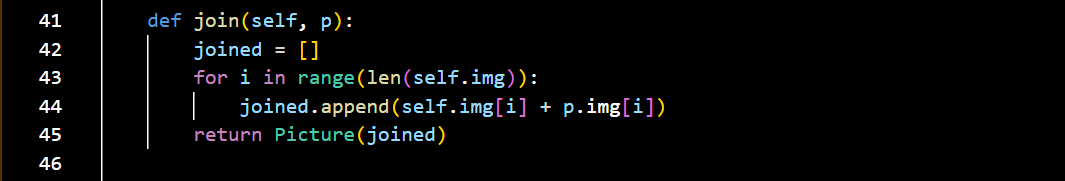
\includegraphics[width=0.8\textwidth,keepaspectratio]{img/join.png}
		%\includesvg{img/automata.svg}
		%\label{img:mot2}
		\caption{Agregando metodo join}
	\end{figure}
	\begin{itemize}	
		\item El metodo join recibe 2 parametros: self y p
		\item El metodo se encarga de juntar las lineas de cadena de String de cada uno y devolver un nuevo objeto Picture
	\end{itemize}

 	\begin{lstlisting}[language=bash,caption={Agregando metodo negative de la clase Picture}][H]
	\end{lstlisting}
	\begin{figure}[H]
		\centering
		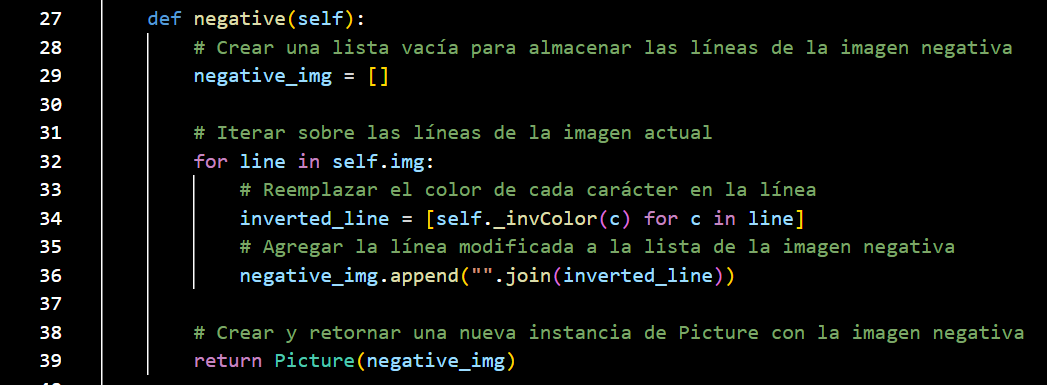
\includegraphics[width=0.8\textwidth,keepaspectratio]{img/negative.png}
		%\includesvg{img/automata.svg}
		%\label{img:mot2}
		\caption{Captura del método negative}
	\end{figure}
	\begin{itemize}	
		\item El metodo negative reemplaza el color de cada linea de la imagen mandada
	\end{itemize}
        \clearpage
	\begin{lstlisting}[language=bash,caption={Completando Ejercicio2a}][H]
		$ git add Ejercicio2a
		$ git commit -m "Completando Ejercicio2a"			
	\end{lstlisting}
	\lstinputlisting[language=Python, caption={Ejercicio2a.py},numbers=left,]{src/Ejercicio2a.py}
	\begin{itemize}	
		\item Se soluciona usando los metodos join y up de la clase Picture
	\end{itemize}
	\begin{figure}[H]
		\centering
		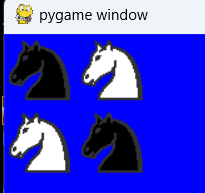
\includegraphics[width=0.4\textwidth,keepaspectratio]{img/2a.png}
		%\includesvg{img/automata.svg}
		%\label{img:mot2}
		\caption{Compilando y probando ejercicicio2a}
	\end{figure}
	\begin{lstlisting}[language=bash,caption={Completando Ejercicio2b}][H]
		$ git add Ejercicio2b
		$ git commit -m "Completando Ejercicio2b"			
	\end{lstlisting}
	\lstinputlisting[language=Python, caption={Ejercicio2b.py},numbers=left,]{src/Ejercicio2b.py}
	\begin{itemize}	
		\item Es similar al ejercicio2a pero en este caso támbien se usa el metodo verticalMirror()
	\end{itemize}
	\begin{figure}[H]
		\centering
		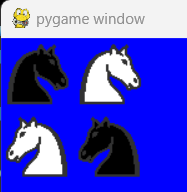
\includegraphics[width=0.4\textwidth,keepaspectratio]{img/2b.png}
		%\includesvg{img/automata.svg}
		%\label{img:mot2}
		\caption{Compilando y probando ejercicicio2b}
	\end{figure}

        \begin{lstlisting}[language=bash,caption={Completando Ejercicio2c}][H]
		$ git add Ejercicio2c
		$ git commit -m "Completando Ejercicio2c"			
	\end{lstlisting}
	\lstinputlisting[language=Python, caption={Ejercicio2c.py},numbers=left,]{src/Ejercicio2c.py}
	\begin{itemize}	
		\item En este ejercicio se hace uso del método horizontalRepeat()
	\end{itemize}
	\begin{figure}[H]
		\centering
		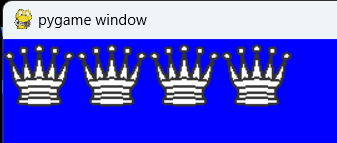
\includegraphics[width=0.4\textwidth,keepaspectratio]{img/2c.png}
		%\includesvg{img/automata.svg}
		%\label{img:mot2}
		\caption{Compilando y probando ejercicicio2c}
	\end{figure}

	\begin{lstlisting}[language=bash,caption={Completando Ejercicio2d}][H]
		$ git add Ejercicio2d
		$ git commit -m "Completando Ejercicio2d"			
	\end{lstlisting}
	\lstinputlisting[language=Python, caption={Ejercicio2d.py},numbers=left,]{src/Ejercicio2d.py}
	\begin{itemize}	
		\item Se usa Picture(SQUARE) para crear el tablero de ajedrez
  		\item Se usa el método horizontal repeat para facilitar el código
	\end{itemize}
	\begin{figure}[H]
		\centering
		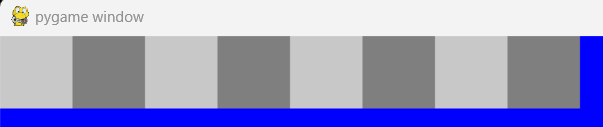
\includegraphics[width=0.4\textwidth,keepaspectratio]{img/2d.png}
		%\includesvg{img/automata.svg}
		%\label{img:mot2}
		\caption{Compilando y probando ejercicicio2d}
	\end{figure}

	\begin{lstlisting}[language=bash,caption={Completando Ejercicio2f}][H]
		$ git add Ejercicio2f
		$ git commit -m "Completando Ejercicio2f"			
	\end{lstlisting}
	\lstinputlisting[language=Python, caption={Ejercicio2f.py},numbers=left,]{src/Ejercicio2f.py}
	\begin{itemize}	
		\item Se usa lo hecho en los ejercicios 2d y 2e   
  		\item Se añade el metodo verticalRepeat()
	\end{itemize}
	\begin{figure}[H]
		\centering
		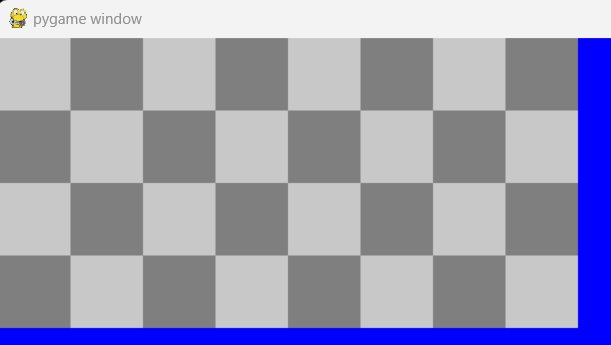
\includegraphics[width=0.4\textwidth,keepaspectratio]{img/2f.png}
		%\includesvg{img/automata.svg}
		%\label{img:mot2}
		\caption{Compilando y probando ejercicicio2f}
	\end{figure}

 	\begin{lstlisting}[language=bash,caption={Agregando metodo overlay de  la clase Picture}][H]		
	\end{lstlisting}
	\begin{itemize}	
		\item El metodo overlay recibe 4 parametros un objeto Picture, una pieza y dos posiciones
  		\item Se usa para colocar las piezas en los espacios del tablero
	\end{itemize}
	\begin{figure}[H]
		\centering
		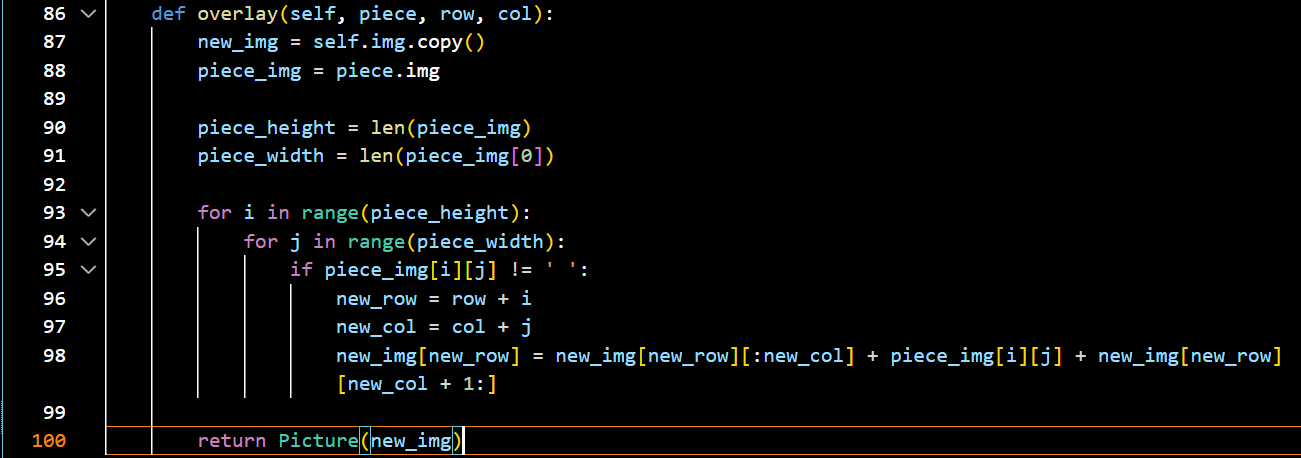
\includegraphics[width=0.4\textwidth,keepaspectratio]{img/overlay.png}
		%\includesvg{img/automata.svg}
		%\label{img:mot2}
		\caption{Agregando metodo overlay}
	\end{figure}
        \clearpage
 	\begin{lstlisting}[language=bash,caption={Completando Ejercicio2g}][H]
		$ git add Ejercicio2g
		$ git commit -m "Completando Ejercicio2g"			
	\end{lstlisting}
	\lstinputlisting[language=Python, caption={Ejercicio2g.py},numbers=left,]{src/Ejercicio2g.py}
	\begin{itemize}	
		\item Se usa el metodo overlay para colocar las piezas en sus espacios correspondientes
  		\item Se usa lo hecho en los ejercicios anteriores
	\end{itemize}
	\begin{figure}[H]
		\centering
		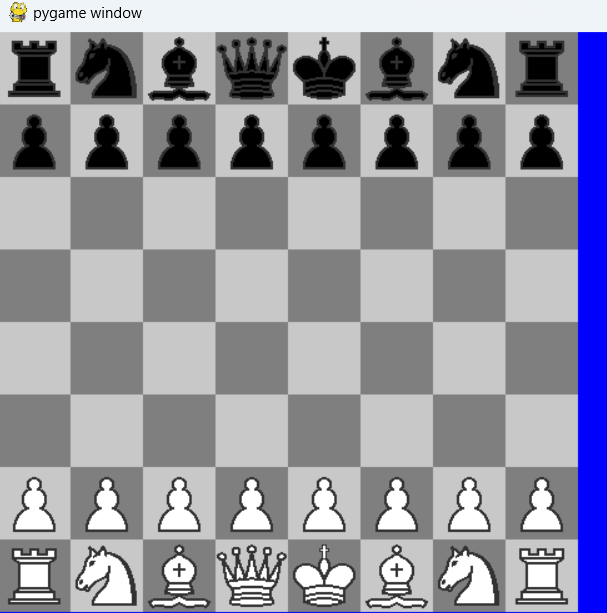
\includegraphics[width=0.4\textwidth,keepaspectratio]{img/2g.png}
		%\includesvg{img/automata.svg}
		%\label{img:mot2}
		\caption{Compilando y probando ejercicicio2g}
	\end{figure}

\section{Cuestionario}
    \subsection{¿Qué son los archivos *.pyc?}
    Los archivos con extensión ".pyc" son archivos de código de byte generados por el intérprete de Python. Cuando se ejecuta un programa de Python, el código fuente se compila en un formato de código de byte, que es más eficiente para ser interpretado por la máquina virtual de Python. Los archivos .pyc contienen esta versión compilada del código fuente y se utilizan para acelerar la carga y ejecución de programas de Python en futuras ocasiones.
    
     \subsection{¿Para qué sirve el directorio pycache?}
El directorio "pycache" es utilizado por el intérprete de Python para almacenar los archivos .pyc generados durante la compilación de código fuente en módulos. Este directorio se crea automáticamente en el mismo directorio que el archivo .py cuando se importa un módulo.

La finalidad del directorio "pycache" es proporcionar un lugar específico para almacenar los archivos .pyc y evitar el desorden en el directorio principal donde se encuentran los archivos .py. Al separar los archivos .pyc en un directorio aparte, se mejora la organización del proyecto y se mantiene más limpio el espacio de trabajo.
     \subsection{¿Cuáles son los usos y lo que representa el subguión en Python?}
    El subrayado o guion bajo tiene diversos usos y significados en Python. En primer lugar, se utiliza como un nombre de variable descartable, cuando se quiere ignorar un valor en un bucle o en una asignación. Además, el subrayado al comienzo de un nombre de variable se emplea como convención para indicar que esa variable es de uso interno y no debe ser accedida directamente desde fuera de la clase o módulo.

	\section{\textcolor{red}{Rúbricas}}
	
	\subsection{\textcolor{red}{Entregable Informe}}
	\begin{table}[H]
		\caption{Tipo de Informe}
		\setlength{\tabcolsep}{0.5em} % for the horizontal padding
		{\renewcommand{\arraystretch}{1.5}% for the vertical padding
		\begin{tabular}{|p{3cm}|p{12cm}|}
			\hline
			\multicolumn{2}{|c|}{\textbf{\textcolor{red}{Informe}}}  \\
			\hline 
			\textbf{\textcolor{red}{Latex}} & \textcolor{blue}{El informe está en formato PDF desde Latex,  con un formato limpio (buena presentación) y facil de leer.}   \\ 
			\hline 
			
			
		\end{tabular}
	}
	\end{table}
	
	\clearpage
	
	\subsection{\textcolor{red}{Rúbrica para el contenido del Informe y demostración}}
	\begin{itemize}			
		\item El alumno debe marcar o dejar en blanco en celdas de la columna \textbf{Checklist} si cumplio con el ítem correspondiente.
		\item Si un alumno supera la fecha de entrega,  su calificación será sobre la nota mínima aprobada, siempre y cuando cumpla con todos lo items.
		\item El alumno debe autocalificarse en la columna \textbf{Estudiante} de acuerdo a la siguiente tabla:
	
		\begin{table}[ht]
			\caption{Niveles de desempeño}
			\begin{center}
			\begin{tabular}{ccccc}
    			\hline
    			 & \multicolumn{4}{c}{Nivel}\\
    			\cline{1-5}
    			\textbf{Puntos} & Insatisfactorio 25\%& En Proceso 50\% & Satisfactorio 75\% & Sobresaliente 100\%\\
    			\textbf{2.0}&0.5&1.0&1.5&2.0\\
    			\textbf{4.0}&1.0&2.0&3.0&4.0\\
    		\hline
			\end{tabular}
		\end{center}
	\end{table}	
	
	\end{itemize}
	
	\begin{table}[H]
		\caption{Rúbrica para contenido del Informe y demostración}
		\setlength{\tabcolsep}{0.5em} % for the horizontal padding
		{\renewcommand{\arraystretch}{1.5}% for the vertical padding
		%\begin{center}
		\begin{tabular}{|p{2.7cm}|p{7cm}|x{1.3cm}|p{1.2cm}|p{1.5cm}|p{1.1cm}|}
			\hline
    		\multicolumn{2}{|c|}{Contenido y demostración} & Puntos & Checklist & Estudiante & Profesor\\
			\hline
			\textbf{1. GitHub} & Hay enlace URL activo del directorio para el  laboratorio hacia su repositorio GitHub con código fuente terminado y fácil de revisar. &2 & & & \\ 
			\hline
			\textbf{2. Commits} &  Hay capturas de pantalla de los commits más importantes con sus explicaciones detalladas. (El profesor puede preguntar para refrendar calificación). &4 & & & \\ 
			\hline 
			\textbf{3. Código fuente} &  Hay porciones de código fuente importantes con numeración y explicaciones detalladas de sus funciones. &2 & & & \\ 
			\hline 
			\textbf{4. Ejecución} & Se incluyen ejecuciones/pruebas del código fuente  explicadas gradualmente. &2 & & & \\ 
			\hline			
			\textbf{5. Pregunta} & Se responde con completitud a la pregunta formulada en la tarea.  (El profesor puede preguntar para refrendar calificación).  &2 & & & \\ 
			\hline	
			\textbf{6. Fechas} & Las fechas de modificación del código fuente estan dentro de los plazos de fecha de entrega establecidos. &2 & & & \\ 
			\hline 
			\textbf{7. Ortografía} & El documento no muestra errores ortográficos. &2 & & & \\ 
			\hline 
			\textbf{8. Madurez} & El Informe muestra de manera general una evolución de la madurez del código fuente,  explicaciones puntuales pero precisas y un acabado impecable.   (El profesor puede preguntar para refrendar calificación).  &4 & & & \\ 
			\hline
			\multicolumn{2}{|c|}{\textbf{Total}} &20 & & & \\ 
			\hline
		\end{tabular}
		%\end{center}
		%\label{tab:multicol}
		}
	\end{table}
	
\clearpage

\section{Referencias}
\begin{itemize}			
	\item \url{https://www.w3schools.com/python/python_reference.asp}
	\item \url{https://docs.python.org/3/tutorial/}
\end{itemize}	
	
%\clearpage
%\bibliographystyle{apalike}
%\bibliographystyle{IEEEtranN}
%\bibliography{bibliography}
			
\end{document}